\documentclass[10pt,aspectratio=149]{beamer}
\usecolortheme{Calm}
\usetheme{Calm}
\usepackage{pgfplots}
\usepackage{pgfplotstable}
\usepackage[utf8]{inputenc}
\usepackage{hyperref}
\RequirePackage[absolute,overlay]{textpos}
%\usepackage[sfdefault]{cabin}
%\usepackage[T1]{fontenc}
%\setlength{\TPHo{}rizModule}{\paperwidth}
%\setlength{\TPVertModule}{\paperheight}
%\definecolor{OQEdarkblue}{HTML}{046085}


\defbeamertemplate*{background canvas}{bg}
{%
  \color{lightgray!40}\vrule width\paperwidth height\paperheight% added bg color
}

% Centered, larger display equation
\newcommand{\keyeq}[1]{%
  \begin{center}
    \Large$\displaystyle #1$
  \end{center}%
}

% Image scaled to height #1, top-aligned in a box of that exact height so that
% side-by-side images of different aspect ratios stay vertically aligned
% (beamer's columns top-aligns on each column's natural content height, which
% otherwise differs once the image is wider/narrower than its column).
\newcommand{\imgcol}[2]{%
  \begin{center}
    \parbox[t][#1][c]{\linewidth}{\centering\includegraphics[height=#1]{#2}}
  \end{center}%
}

%------------------------------

\author{Dominique Gravel}
\title{From individuals to collective behaviour}
\date{August 24th, 2026}
\institute{Université de Sherbrooke \\ Summer school in biodiversity modelling}

%------------------------------
% TITLE SLIDE
%------------------------------

\usebackgroundtemplate
{
  
\includegraphics[width=\paperwidth,height=\paperheight]{bg}%
}

\begin{document}

	\begin{frame}[plain]
		\titlepage
	\end{frame}

%------------------------------
% INTRODUCTION
%------------------------------

\begin{frame}

	\begin{columns}
		\begin{column}{0.5\textwidth}
            \begin{center}
                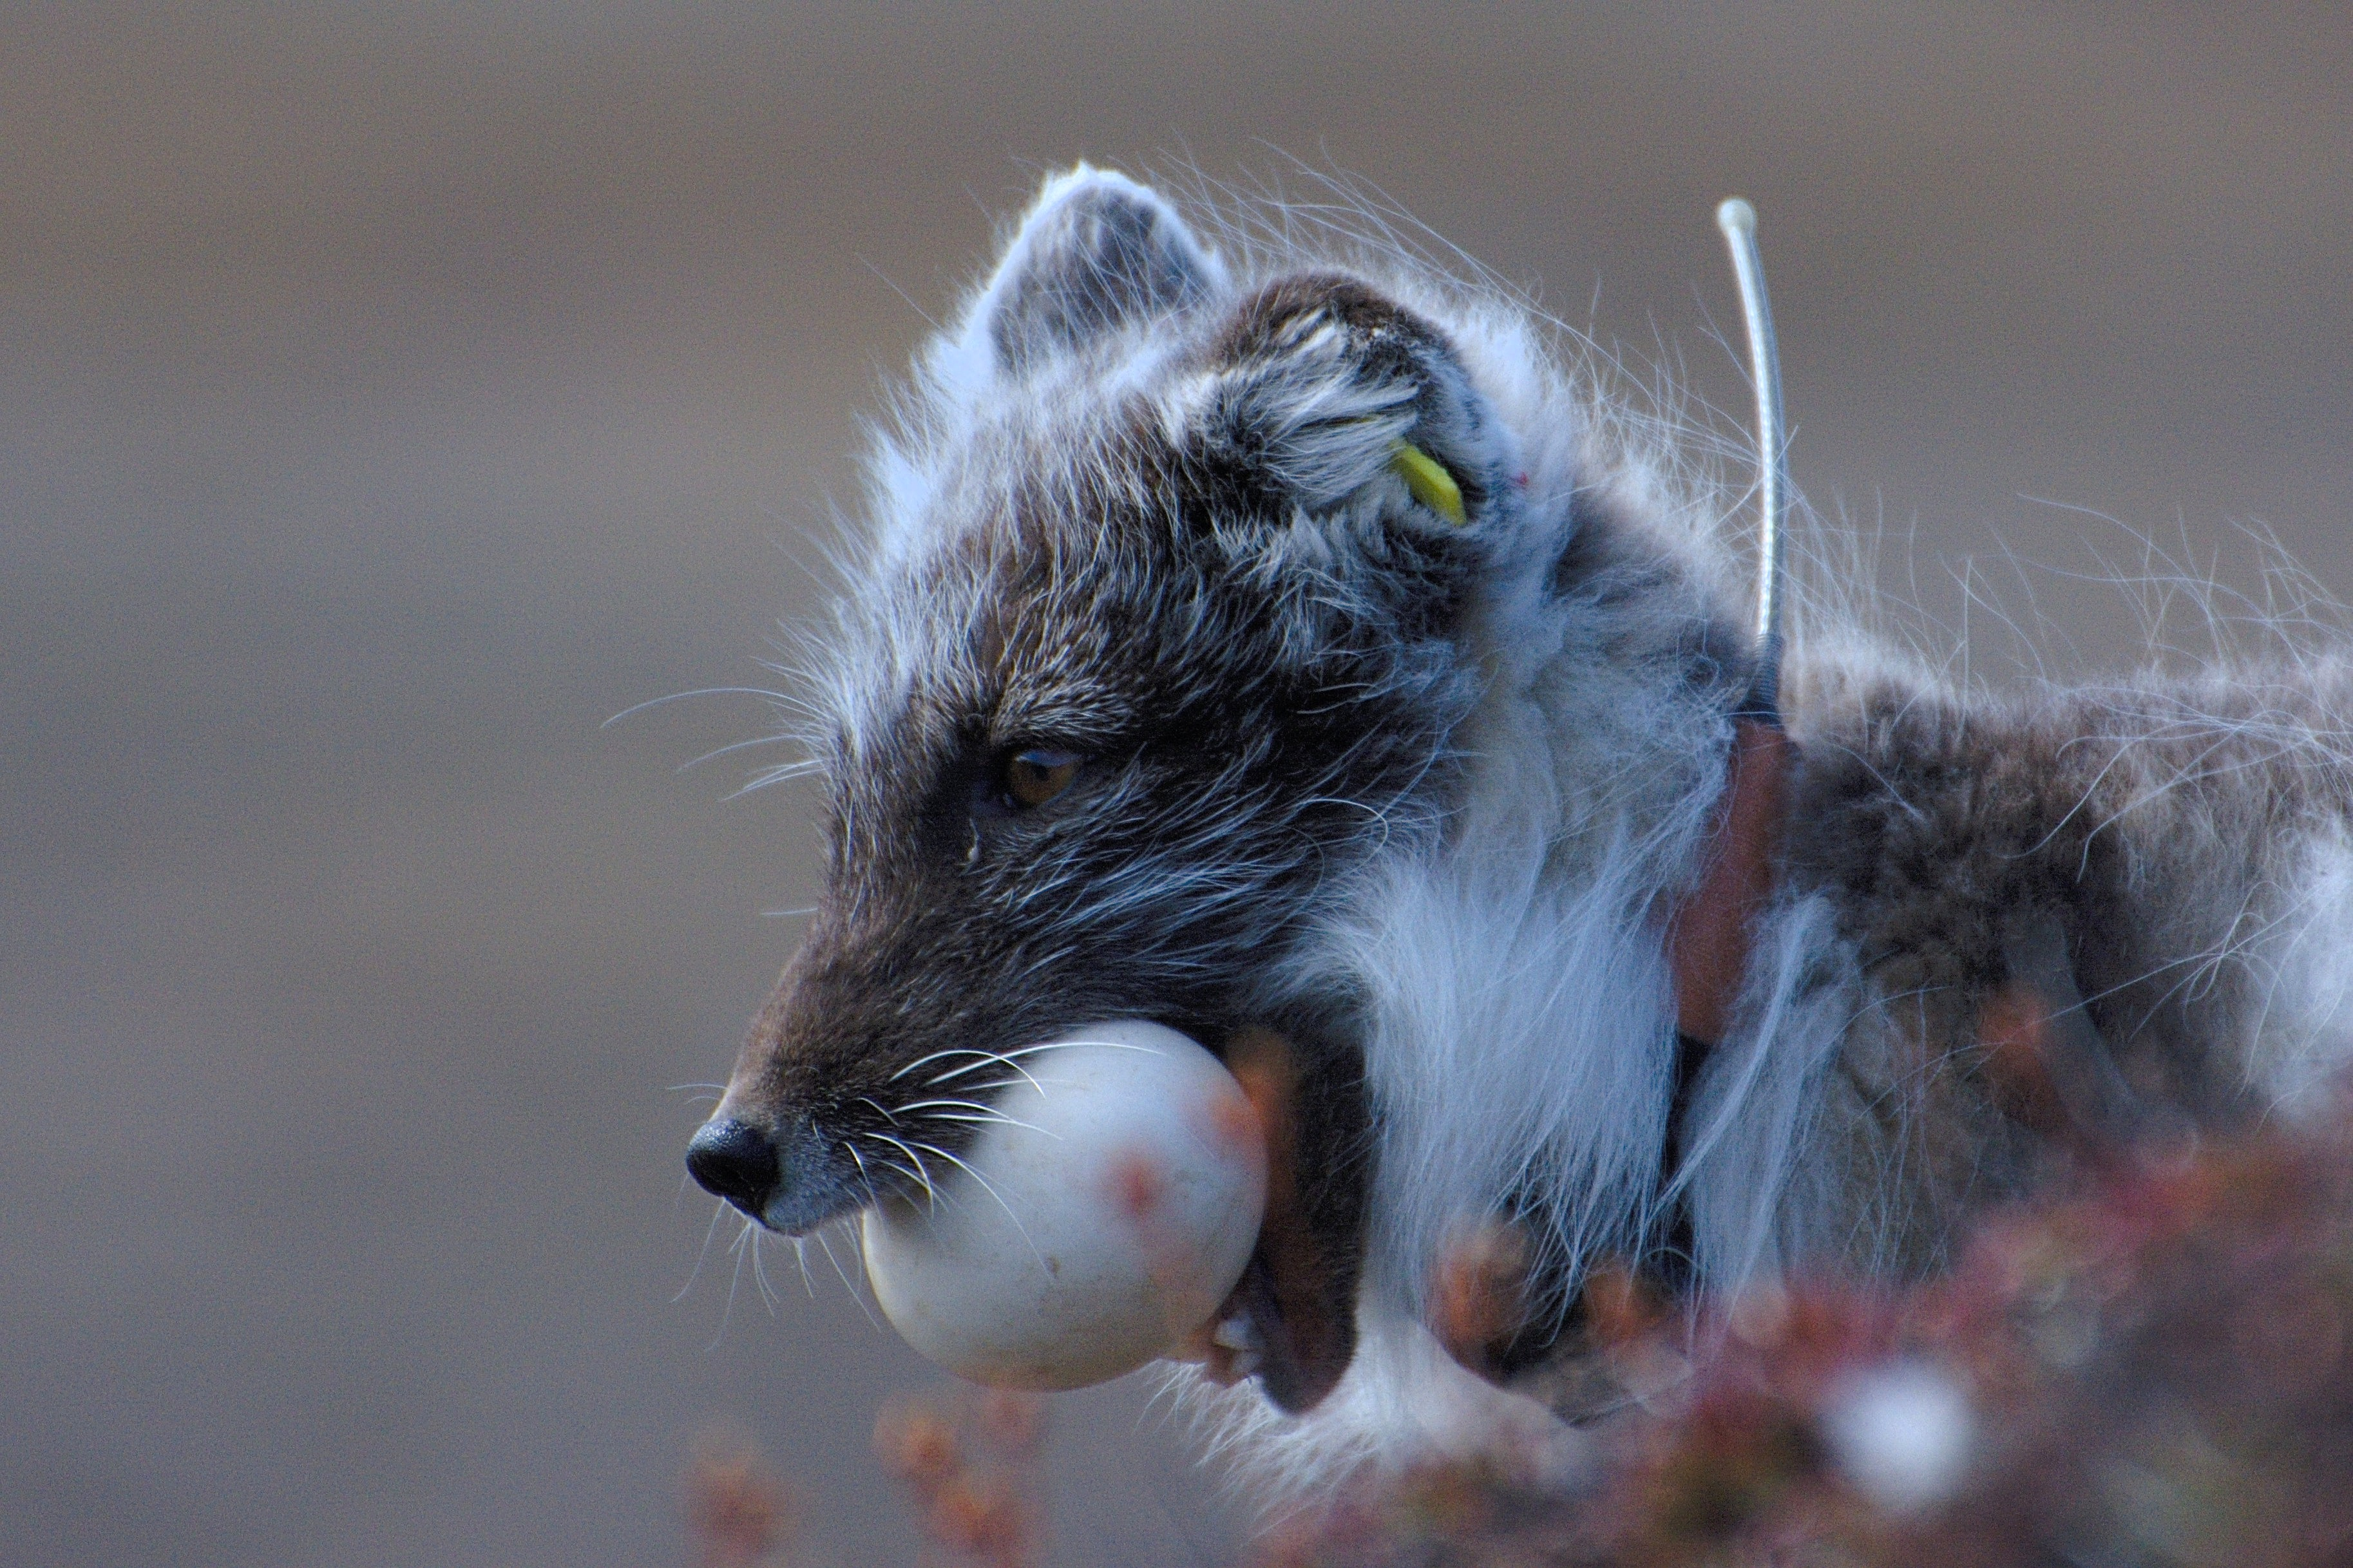
\includegraphics[height=0.5\textheight]{Figs/fox}
            \end{center}
		\end{column}
%----
		\begin{column}{0.5\textwidth}	

		\end{column}				
	\end{columns} 

\end{frame}

%------------------------------

\begin{frame}

	\begin{columns}
		\begin{column}{0.5\textwidth}
            \imgcol{0.5\textheight}{Figs/fox}
		\end{column}
%----
		\begin{column}{0.5\textwidth}
            \imgcol{0.5\textheight}{Figs/telemetry}
		\end{column}
	\end{columns}

\end{frame}

%------------------------------

\begin{frame}{Statistical analysis}

	\begin{columns}
		\begin{column}{0.5\textwidth}
            \imgcol{0.5\textheight}{Figs/fox}
		\end{column}
%----
		\begin{column}{0.5\textwidth}
            \imgcol{0.5\textheight}{Figs/dulude2023}
		\end{column}
	\end{columns}

\end{frame}

%------------------------------

\begin{frame}{Resource-selection function}

    \begin{center}
        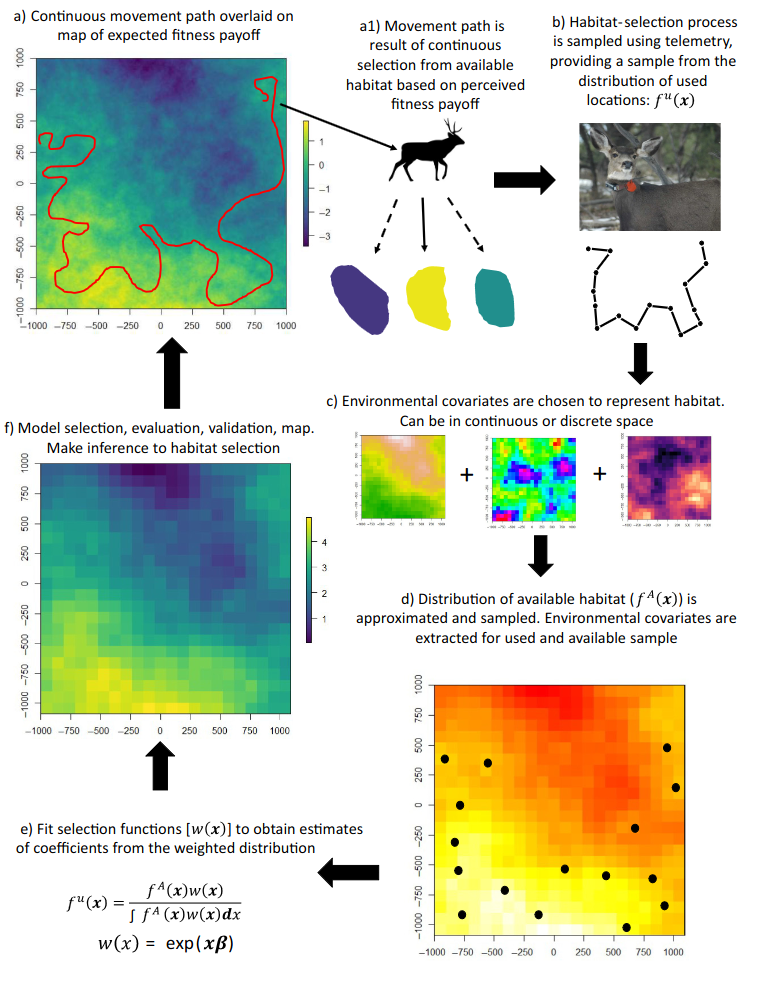
\includegraphics[height=0.7\textheight]{Figs/northrup2022}
    \end{center}

\end{frame}

%------------------------------

\begin{frame}{Outline}

    \begin{itemize}
        \item Random walk and diffusion 
        \item Mechanistic home range analysis
        \item Adding population dyanmics
        \item Predator-prey interactions
        \item Self-organization \& complex spatial structures
    \end{itemize}

\end{frame}

%------------------------------
% EXERCISE
%------------------------------

{
\usebackgroundtemplate{}
\begin{frame}

	\pagecolor{BDQC1st}
	\color{white}

	\LARGE{\textit{Exercise}}

\end{frame}
}

%------------------------------

\begin{frame}{A minimal individual-based model}

    \begin{itemize}
        \item Start at position (0,0)
        \item At each time step add $\Delta x = \eta(0, \sigma)$ and $\Delta y = \eta(0, \sigma)$
        \item Record position at time $t={1,2,4,6,8,16,32,64}$ time steps
        \item Repeat 100 times
        \item Plot the mean and variance of distance to the center as a function of time
    \end{itemize}

\end{frame}

%------------------------------
% DIFFUSION
%------------------------------

{
\usebackgroundtemplate{}
\begin{frame}

	\pagecolor{BDQC1st}
	\color{white}

	\LARGE{\textit{Theory}}

\end{frame}
}

%------------------------------
\begin{frame}{Random walk}

\textbf{Definition :} a stochastic process that describes a path that consists of a succession of random steps on some mathematical space

    \begin{center}
        \includegraphics[height=0.6\textheight]{Figs/Case_2_1}
    \end{center}

\footnotesize Case, T.J. 2001. An Illustrated guide to theroetical ecology. Oxford University Press \\ Moorcroft and Lewis. 2006. Mechanistic Home Range Analysis. Princeton University Press.

\end{frame}

%------------------------------

\begin{frame}{Diffusion}

    \textbf{Definition :} the population of consequence of many individuals simultaneously undergoing random walks in continuous time and across continuous space
    
        \begin{center}
            \includegraphics[height=0.6\textheight]{Figs/Case_2_2}
        \end{center}
    
    \end{frame}
    
%------------------------------

\begin{frame}{Numerical example}

    \begin{itemize}
        \item Start with $N = 2000$
        \item Each time step, $1/10$ individuals ($d = 0.1$) move to the left and the same to the right
    \end{itemize}
    
    \begin{table}[]
        \begin{tabular}{lllllll}
                   & x=1 & x=2 & x=3  & x=4  & x=5 & x=6 \\
            Time 0 &     &     & 1000 & 1000 &     &     \\
            Time 1 &     & 100 & 900  & 900  & 100 &     \\
            Time 2 & 10  & 170 & 820  & 820  & 170 & 10 
        \end{tabular}
    \end{table}  
    
\end{frame}
    
%------------------------------

\begin{frame}{More generally}

    Density change per cell follows : 

    \keyeq{N_{x, t+1} = N_{x, t} + dN_{x-1, t} + dN_{x+1, t} - 2dN_{x, t}}
    
\end{frame}
    
%------------------------------

\begin{frame}{Result}

    Which looks like : 

    \begin{center}
        \includegraphics[height=0.5\textheight]{Figs/Case_2_5}
    \end{center}
    
\end{frame}
    
%------------------------------

\begin{frame}{From discrete to continuous}

    We can reformulate the equation as a change in density at location $x$ : 

    \keyeq{\Delta N_{x,t}= N_{x, t+1}-N_{x, t} = d[(N_{x-1, t}-N_{x, t}) + (N_{x+1, t}-N_{x, t})]}
    
    As the time and spatial steps get smaller, the formula becomes : 
    
    \keyeq{\frac{dN(x,t)}{dt} = D \frac{\partial^2N(x,t)}{\partial^2 x}}
    
    Where : 
    \begin{itemize}
        \item The left term is the rate at which the density at position $x$ is changing over time
        \item $D$ is the diffusion parameter
        \item The right term is a density gradient at location $x$
    \end{itemize}
    
\end{frame}
    
%------------------------------

\begin{frame}{Diffusion coefficient}

    Units are $distance^2$ per time

    Interpretation is the mean square displacement (one dimension): 
    
    \keyeq{D = \frac{\overline{\delta^2}}{2t}}
    
\end{frame}
    
%------------------------------

\begin{frame}{Solution}

    The number of individuals relased at a location will follow a normal distribution : 

    \keyeq{N(x,t) = \frac{N_0}{\sqrt{4\pi D t}}\exp\left(\frac{-(x-\overline{x})^2}{4Dt}\right)}
    
    With interpretation : 
    \begin{itemize}
        \item The mean displacement expands across space at a rate proportional to the square root of time
        \item The total area (range size) increases proportionnally with time
    \end{itemize}
    
\end{frame}
    
%------------------------------

\begin{frame}{Adding advection}

    \keyeq{\frac{dN(x.t)}{dt} = \underbrace{- \triangledown CN(x,t)}_{advection} + \underbrace{\triangledown^2 DN(x,t)}_{diffusion}}

    Where $\triangledown$ is a short notation for the partial derivative of position over space and $c$ is the advection rate


\end{frame}

%------------------------------
% INCREASING COMPLEXITY IN HOME RANGE
%------------------------------

{
\usebackgroundtemplate{}
\begin{frame}

	\pagecolor{BDQC1st}
	\color{white}

	\LARGE{\textit{Exercise}}

\end{frame}
}

%------------------------------

\begin{frame}{A minimal individual-based model}{Adding a den site}

    What happens if movement changes as the animal gets further away from the den ?

\end{frame}

%------------------------------
% HOME RANGE ANALAYSIS
%------------------------------

{
\usebackgroundtemplate{}
\begin{frame}

	\pagecolor{BDQC1st}
	\color{white}

	\LARGE{\textit{Back to theory}}

\end{frame}
}

%------------------------------
\begin{frame}{Red fox telemetry}

    \begin{center}
        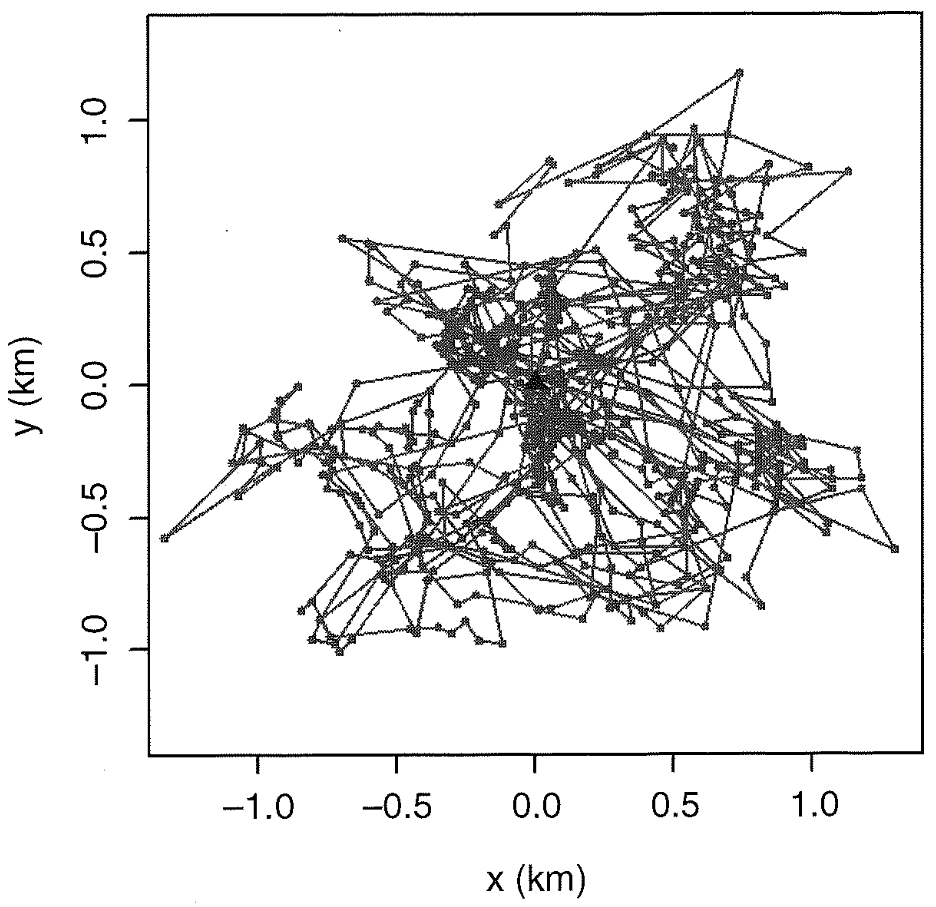
\includegraphics[height=0.7\textheight]{Figs/moorcroft_3_4}
    \end{center}
    
\end{frame}
    
%------------------------------

\begin{frame}{Mechanistic home range analysis}

    \begin{center}
        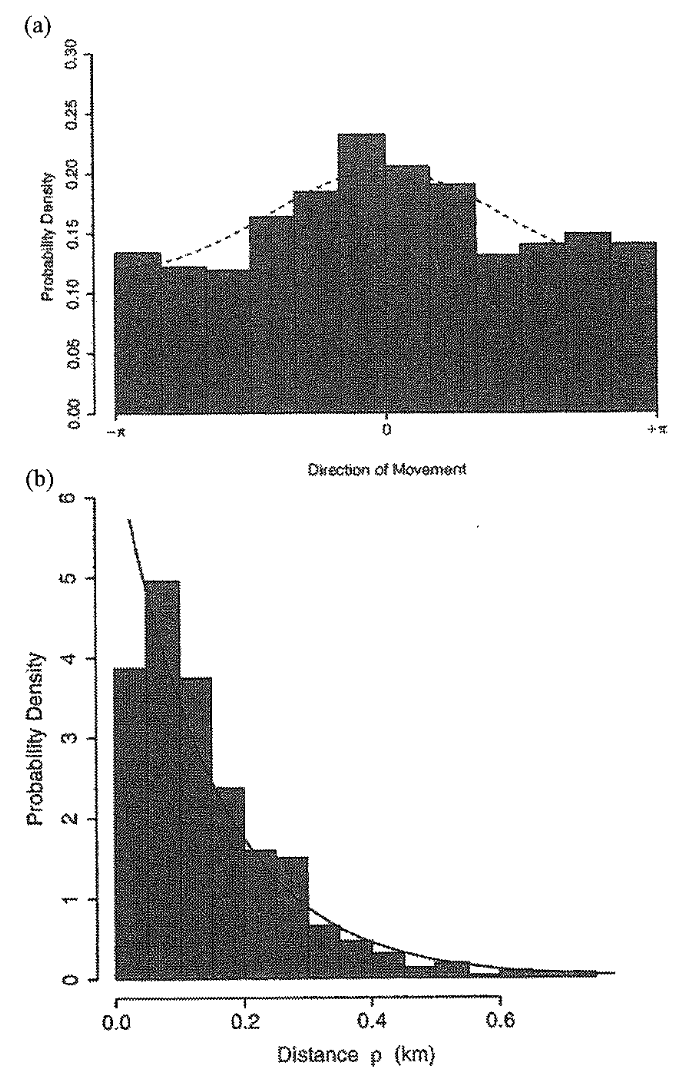
\includegraphics[height=0.7\textheight]{Figs/moorcroft_3_6}
    \end{center}
    
\end{frame}
    
%------------------------------

\begin{frame}{Redistribution kernel}

    The probability density function describing movement from location $x$ to $x'$ : 

    \keyeq{k(x,x',\tau,t) = \frac{1}{\rho}(\rho)K_{\tau}(\phi,\widehat{\phi})}
    
    where 
    \begin{itemize}
        \item $\rho$ is the distance between locations
        \item $\phi$ is the angle between starting point and finishing point
        \item $\widehat{\phi}$ is the direction of the home range center from the current position
    \end{itemize}
    
\end{frame}
    
%------------------------------

\begin{frame}{Redistribution kernel}

    \begin{center}
        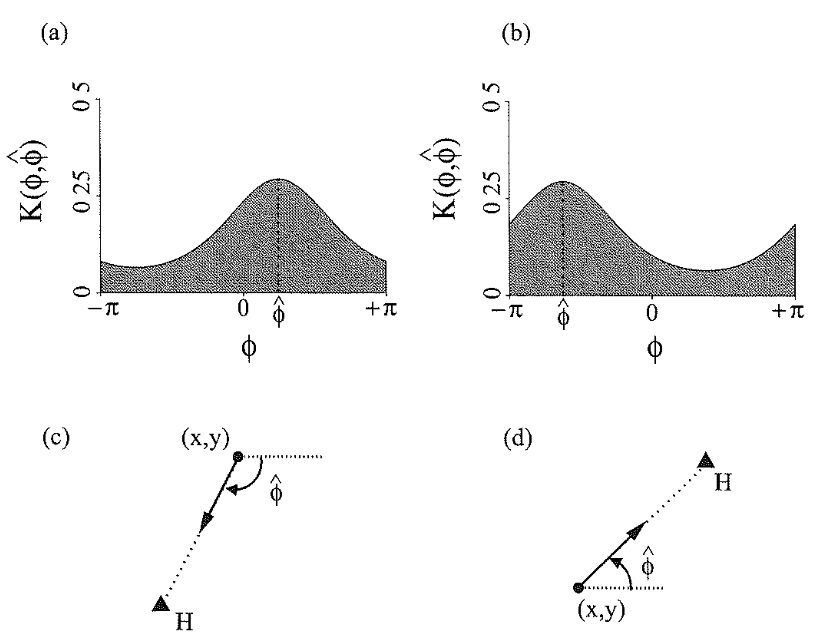
\includegraphics[height=0.7\textheight]{Figs/moorcroft_3_3}
    \end{center}
    
\end{frame}
    
%------------------------------

\begin{frame}{Equation for space use}

    We can revisit the equation for advection-diffusion and compute parameters from the redistribution kernel (hidding complications with 2 dimensions): 

    \keyeq{\frac{dN(x.t)}{dt} = \underbrace{- \triangledown CN(x,t)}_{advection} + \underbrace{\triangledown^2 DN(x,t)}_{diffusion}}
    
    where : 
    
    \begin{itemize}
        \item $C = \kappa_{\tau}\overline{\rho}_{\tau}/2\tau$
        \item $D = \overline{\rho}_{\tau}^2/4\tau$
    \end{itemize}
    
    At equilibrium : diffusion equals advection (movement toward the center of the home range)
    
\end{frame}
    
%------------------------------

\begin{frame}{Solving for home range}

    After a bit of (tedious) maths, we get a fairly simple solution : 

    \keyeq{N(x) = \frac{\beta}{2}\exp(-\beta|x|)}
    
    where $\beta = C/D$
        
\end{frame}
    
%------------------------------

\begin{frame}{Solving for home range}

    \begin{center}
        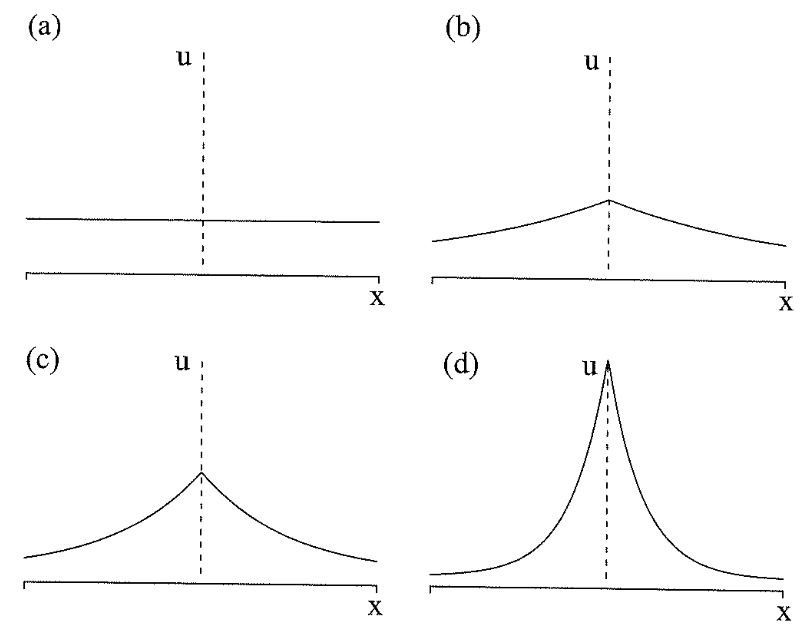
\includegraphics[height=0.6\textheight]{Figs/moorcroft_3_7}
    \end{center}

    For a) $\beta = 0$, b) $\beta = 1$, c) $\beta = 2$ and d) $\beta = 5$.

    Note that the same results hold quantitatively for 2 dimensions. 

\end{frame}
    
%------------------------------

\begin{frame}{Solving for home range}

    We now have a probability density function emerging from first principales and basic statistical descriptors of movement : 

    \begin{center}
        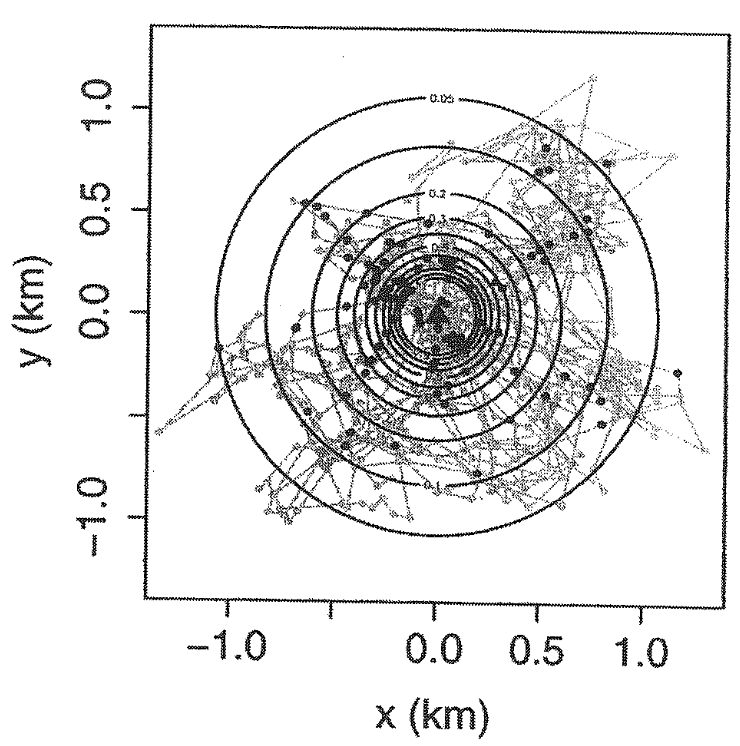
\includegraphics[height=0.6\textheight]{Figs/moorcroft_3_8}
    \end{center}

\end{frame}
    
%------------------------------
% ADDING POPULATION DYNAMICS
%------------------------------

\begin{frame}{Movement plus geometric growth}

    Recall the original discrete time discrete space equation : 

    \keyeq{N_{x, t+1} = N_{x, t} + dN_{x-1, t} + dN_{x+1, t} - 2dN_{x, t}}
    
    And now add geometric growth : 
    
    \keyeq{N_{x, t+1} = rN_{x, t} + dN_{x-1, t} + dN_{x+1, t} - 2dN_{x, t}}
    
    What's your intuition ? 

\end{frame}
    
%------------------------------

\begin{frame}{Movement plus geometric growth}

    \begin{center}
        \includegraphics[height=0.6\textheight]{Figs/Case_2_8}
    \end{center}

\end{frame}
    
%------------------------------

\begin{frame}{Movement plus geometric growth}

    Solution is 

    \keyeq{Radius^2(t) = 4Dt[rt + \ln N_0]}

    Which means :

    \begin{itemize}
        \item Range size ($m^2$) increases proportional to time 
        \item Range limit ($m$) moves proportional to $\sqrt{r}$ and $\sqrt{D}$
    \end{itemize}

\end{frame}
    
%------------------------------

\begin{frame}{Invasive muskrats}{Skellam, 1951}

    \begin{center}
        \includegraphics[height=0.7\textheight]{Figs/Case_2_10}
    \end{center}

\end{frame}

%------------------------------
% PREDADTPOR-PREY INTERACTIONS
%------------------------------

\begin{frame}

    \begin{center}
        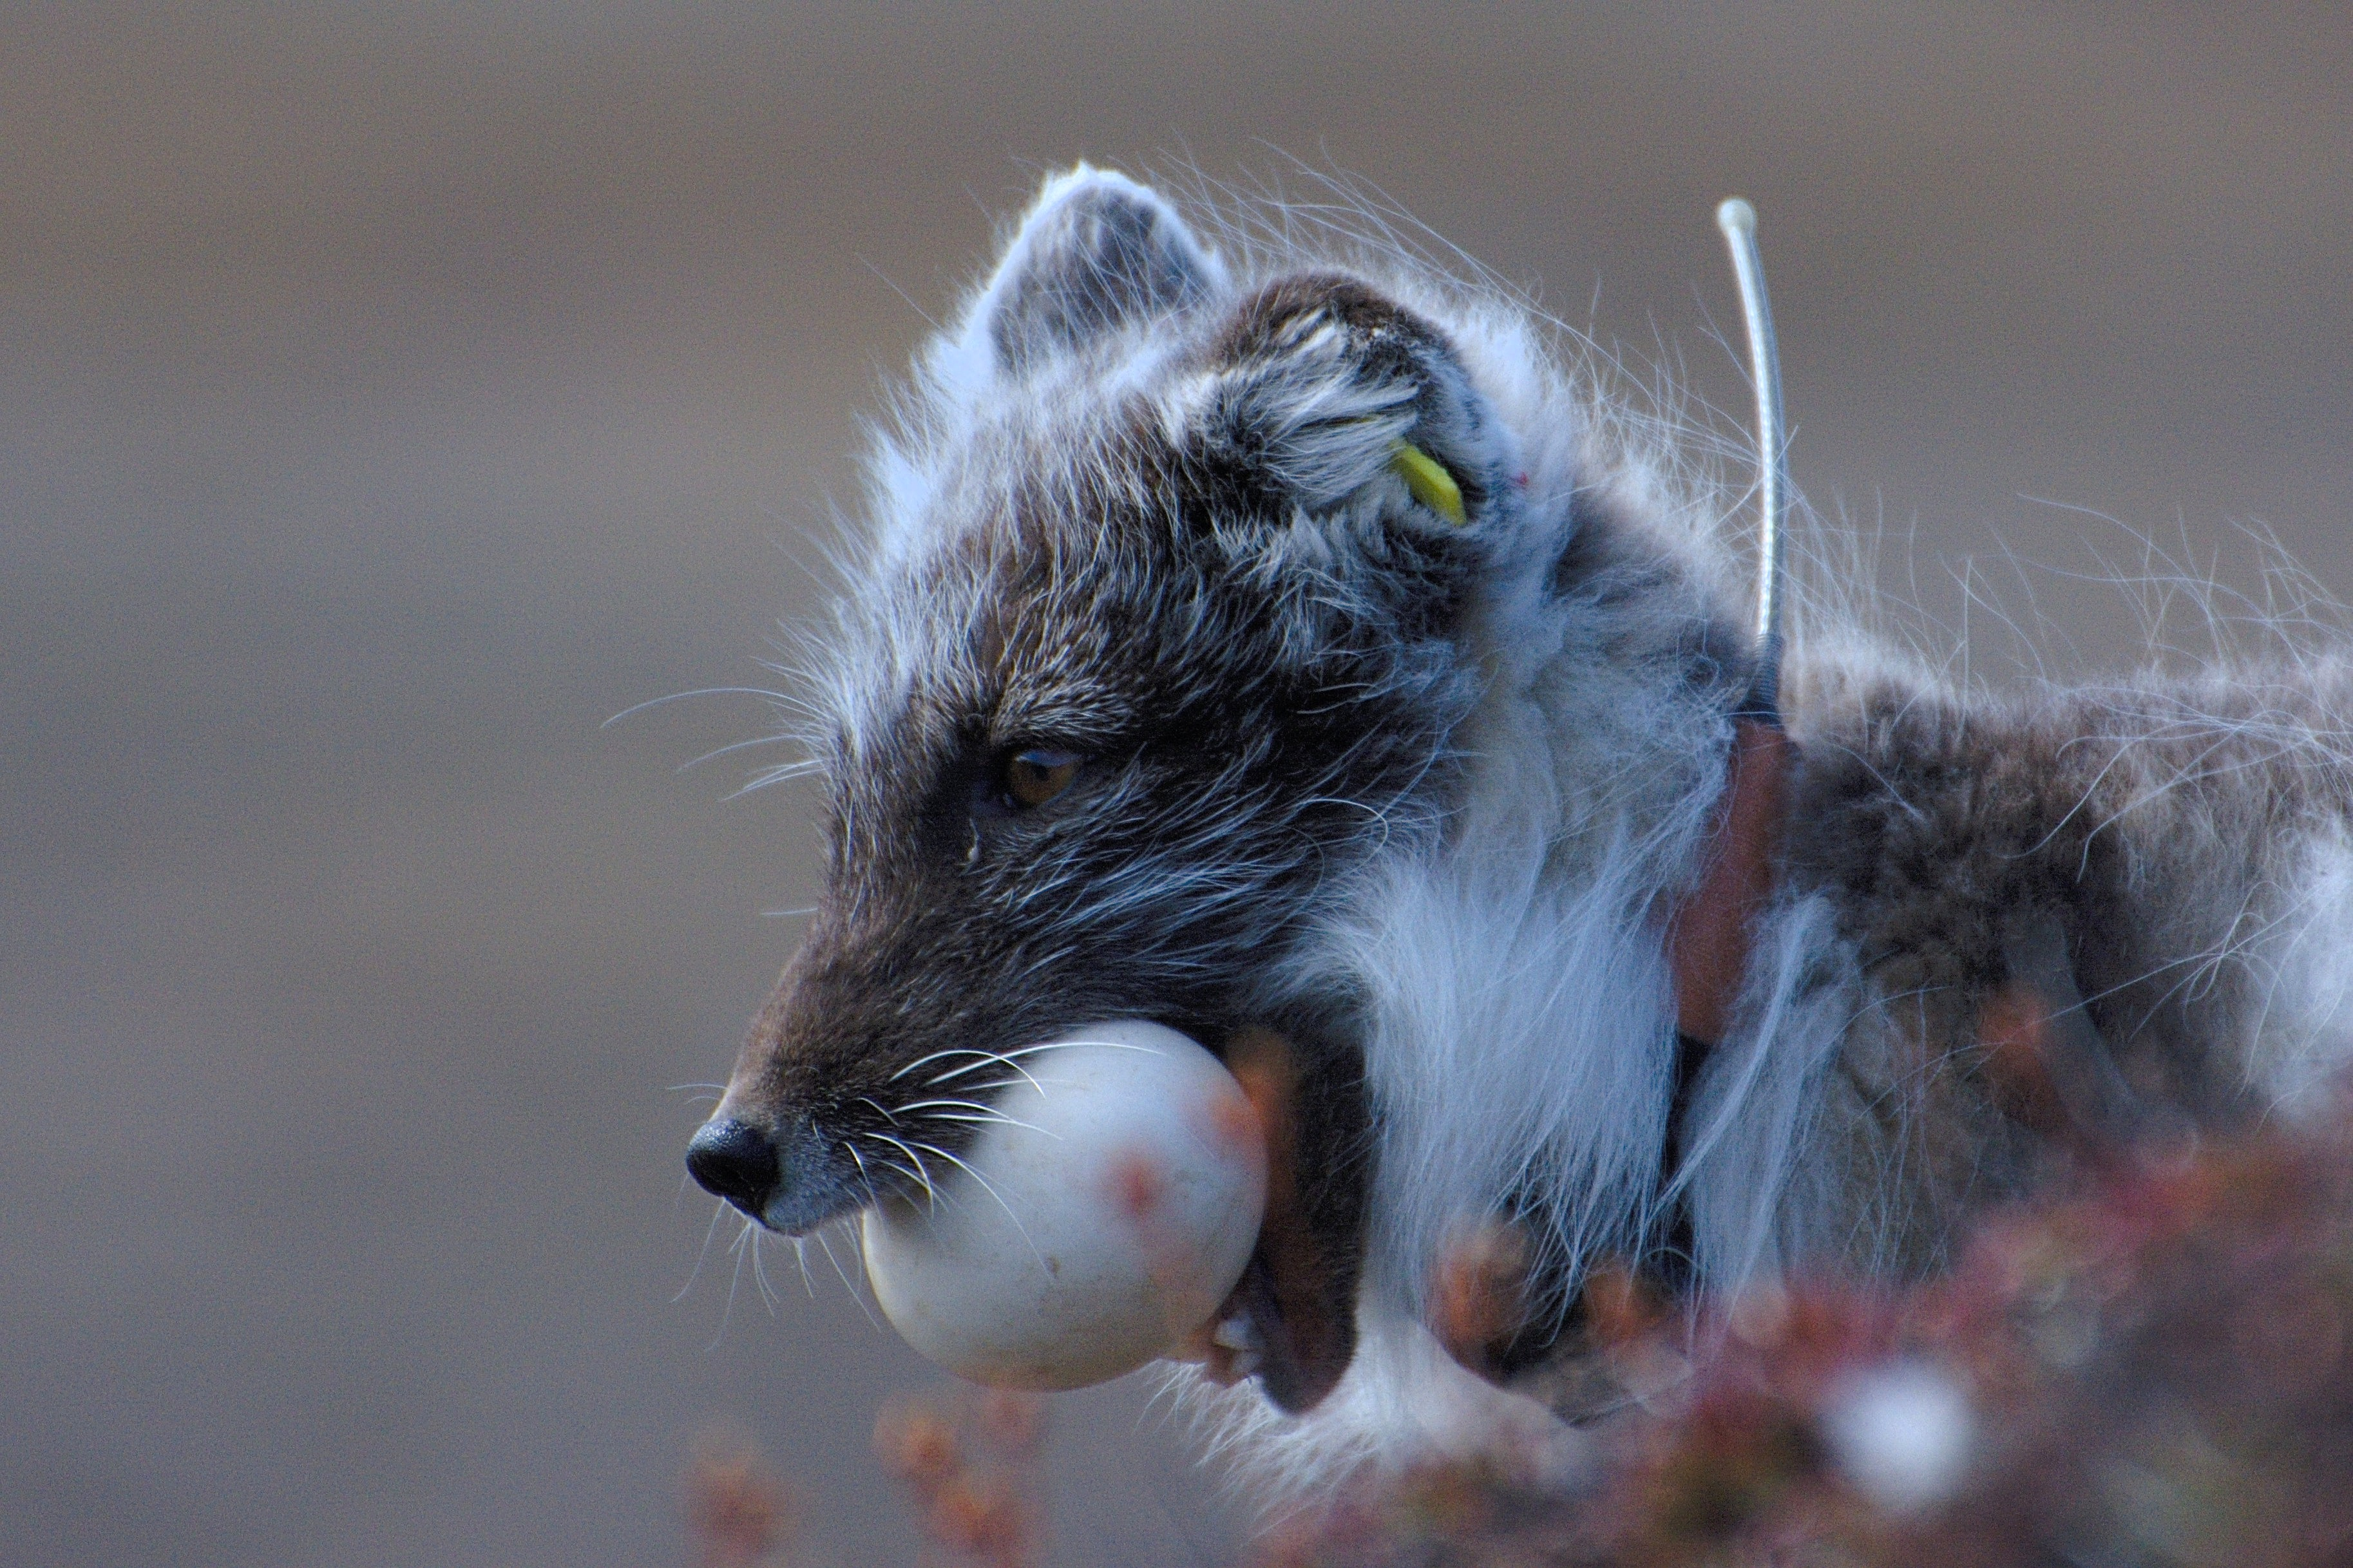
\includegraphics[height=0.6\textheight]{Figs/fox}
    \end{center}

\end{frame}
    
%------------------------------

\begin{frame}{A mechanistic approach}

    \begin{center}
        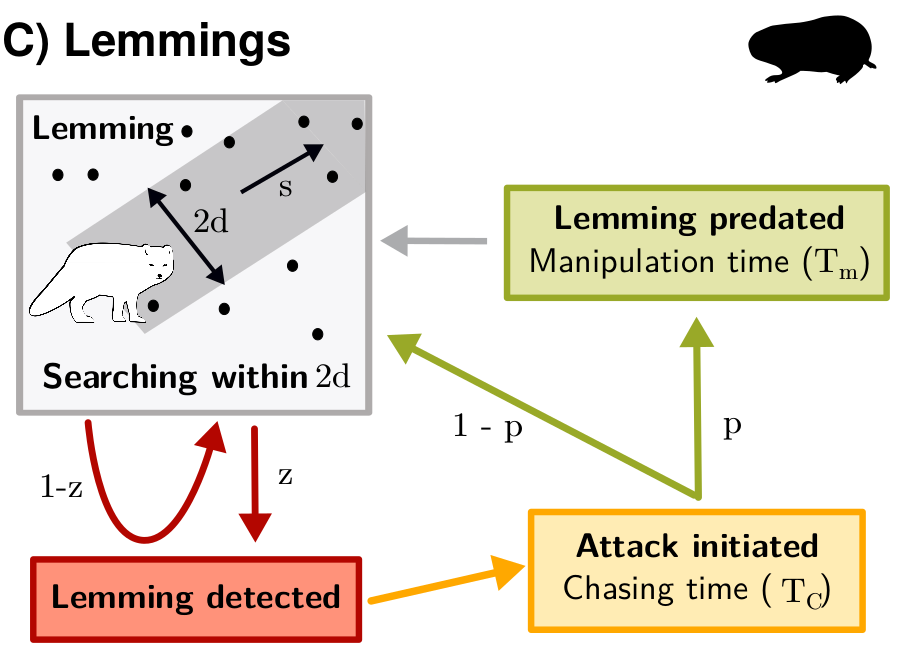
\includegraphics[height=0.6\textheight]{Figs/beardsell2022a}\\
        \footnotesize Beardsell et al. 2022. Front. Ecology
    \end{center}

\end{frame}
    
%------------------------------

\begin{frame}{Law of mass action}

    \textbf{Principle} : predator and prey are randomly moving particles, an interaction occurs whenever a predator encounters a prey, detect it and attack it with success

    The *capture efficiency* ( $km^2/time$ ) of predator individual (or species) $i$ is : 
    
    \keyeq{\alpha_i = s_iz_ik_ip_i}
    
    Where 
    \begin{itemize}
        \item $s_i$ is average movement rate ($km/time$)
        \item $z_i$ is reaction radius ($km$)
        \item $k_i$ is detection probability
        \item $p_i$ is attack probability
    \end{itemize}

    \textbf{Note} : we need to consider both the movement rate of the predator and the prey when both are moving in space

\end{frame}
    
%------------------------------

\begin{frame}{Available time for search}

    \textbf{Principle} : predators need time to catch, consume and process prey. This time is not available for foraging, thereby reducing search efficiency. 

    The \textit{handling time} is the time required to catch and process a prey. It is split into two components : 

    \begin{itemize}
        \item Time spent searching $\frac{T_{ci}}{p_i}$
        \item Time spent manipulating prey $T_{mi}$
    \end{itemize}

    Which yields : 

    \keyeq{h_i = \frac{T_{ci}}{p_i} + T_{mi}}

\end{frame}
    
%------------------------------

\begin{frame}{Integrating the whole thing }

    Putting pieces together we get the famous Holling Type II functional response that we will challenge this week : 

    \keyeq{f(i) = \frac{\alpha_iN_j}{1+\alpha_ih_iN_i}}

\end{frame}
    
%------------------------------

\begin{frame}{Application for the Arctic fox}

    \begin{center}
        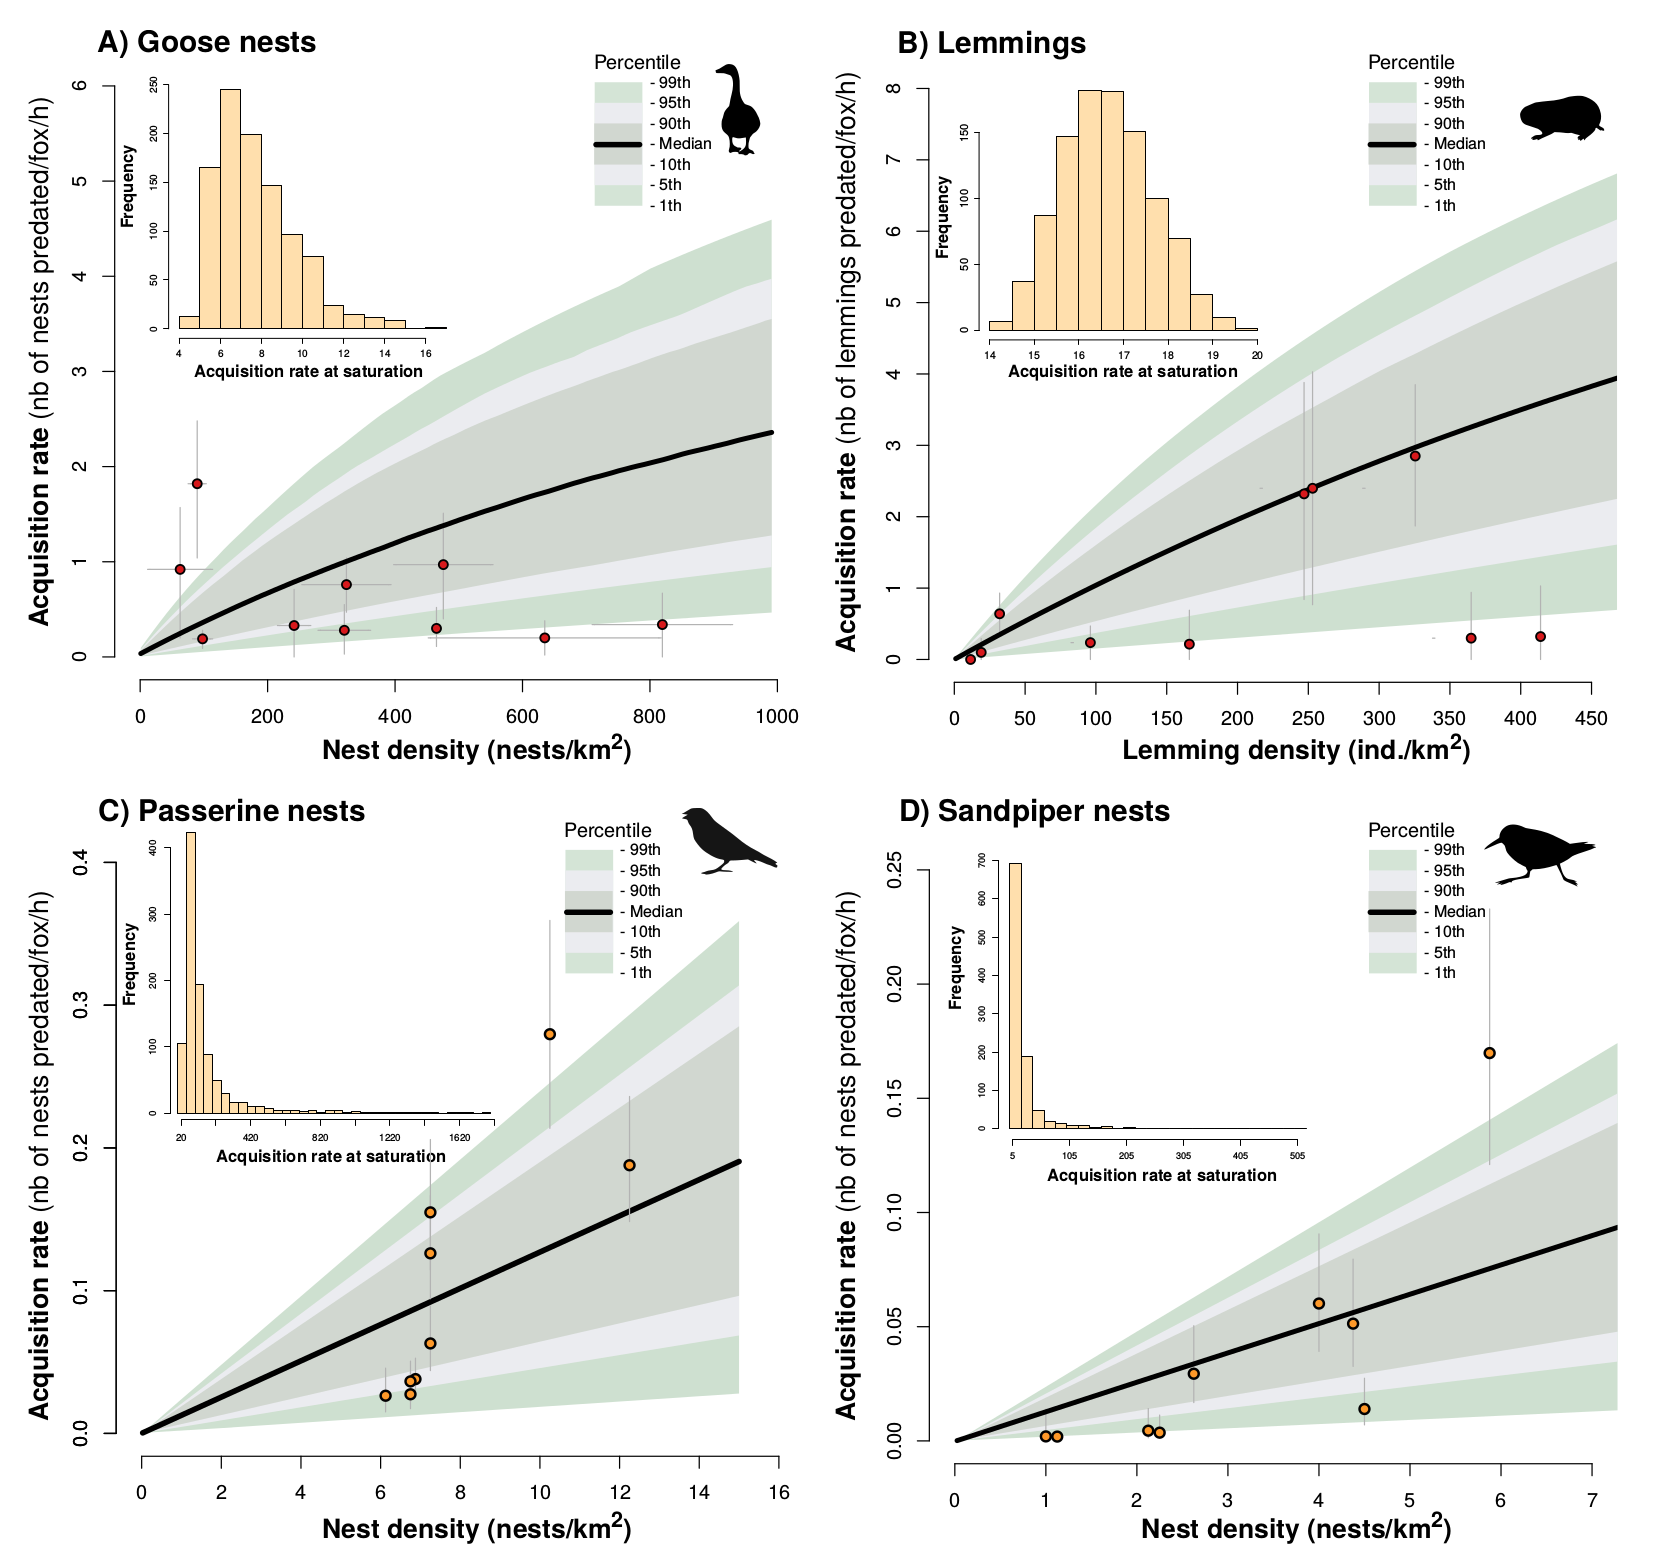
\includegraphics[height=0.6\textheight]{Figs/beardsell2022b}\\
        \footnotesize Beardsell et al. 2022. Front. Ecology
    \end{center}

\end{frame}
    
%------------------------------

\begin{frame}{Non-stationary movement}

    \begin{center}
        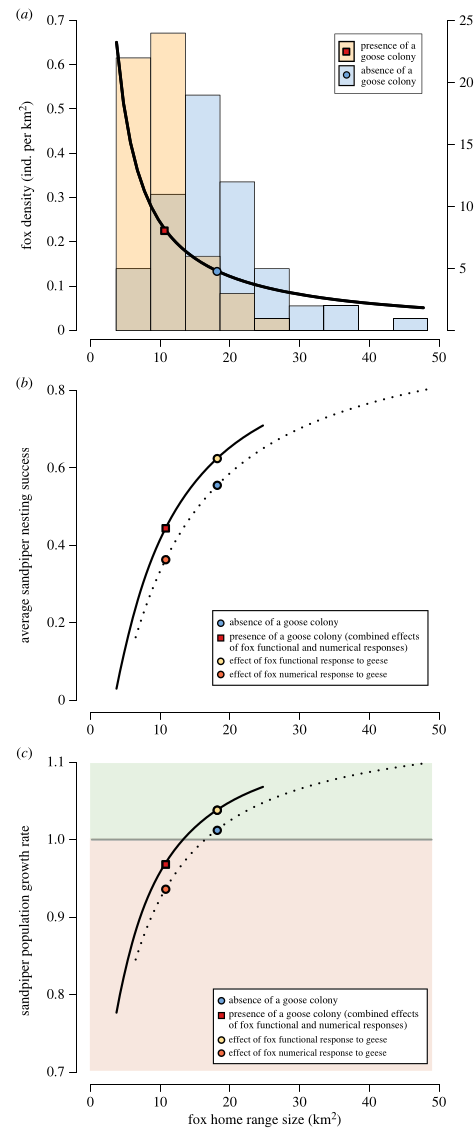
\includegraphics[height=0.7\textheight]{Figs/beardsell2025}\\
        \footnotesize Beardsell et al. 2023. Proc. Roy. Soc. London B.
    \end{center}

\end{frame}
    
%------------------------------

\begin{frame}{Non-random movement}

    \begin{center}
        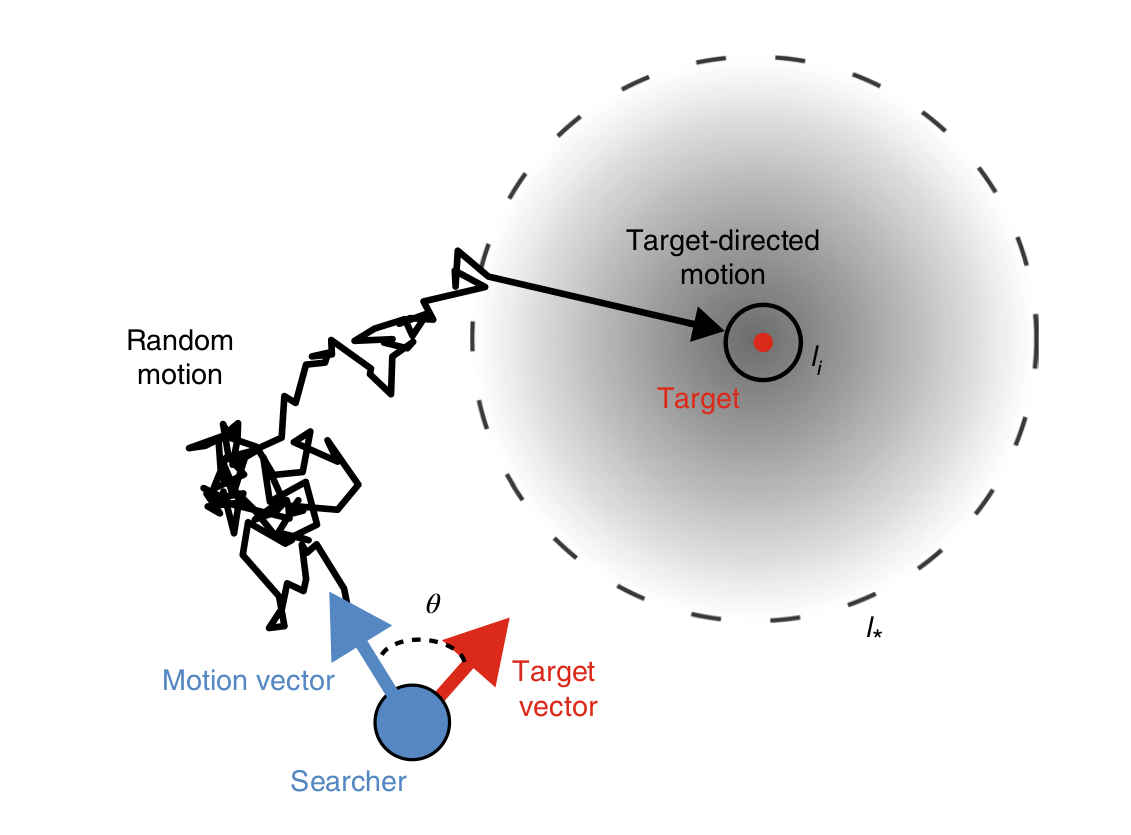
\includegraphics[height=0.6\textheight]{Figs/hein2022}\\
        \footnotesize Hein et al. 2022. Nat. Eco. Evo.
    \end{center}

\end{frame}
    
%------------------------------

\begin{frame}{Dimensionality}

    \begin{center}
        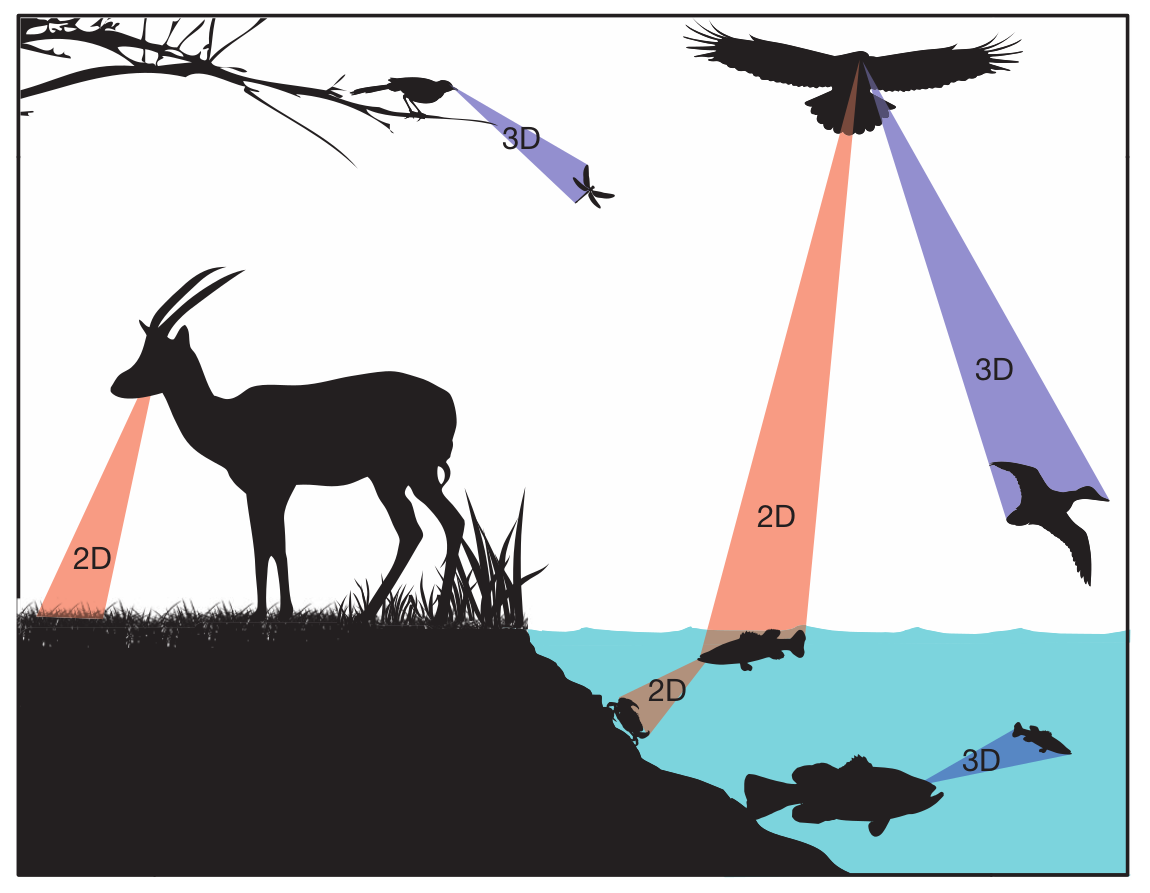
\includegraphics[height=0.6\textheight]{Figs/pawar2012}\\
        \footnotesize Pawar et al. 2012. Nature
    \end{center}

\end{frame}
    
%------------------------------
%  Self-organization \& complex spatial structures
%------------------------------

\begin{frame}{Patch formation in arid ecosystems }

	\begin{columns}
		\begin{column}{0.5\textwidth}
            \begin{center}
                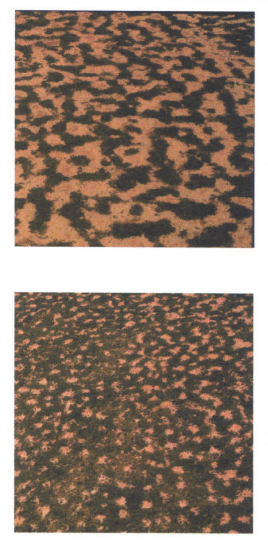
\includegraphics[height=0.6\textheight]{Figs/rietkerk2002a}\\
            \end{center}
		\end{column}
%----
		\begin{column}{0.5\textwidth}	
            \begin{center}
                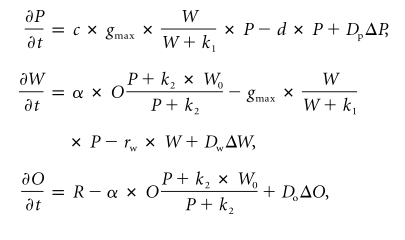
\includegraphics[height=0.4\textheight]{Figs/rietkerk2002b}\\
            \end{center}
		\end{column}				
	\end{columns} 
    \footnotesize Rietkerk et al. 2002. Am. Nat

\end{frame}

%------------------------------

\begin{frame}{Patch formation in arid ecosystems }

	\begin{columns}
		\begin{column}{0.5\textwidth}
            \begin{center}
                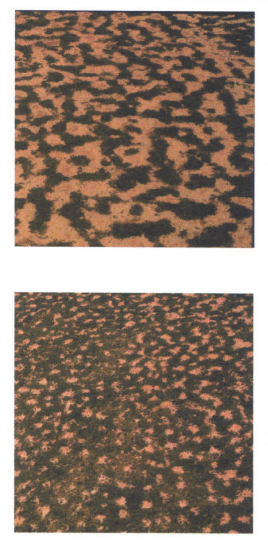
\includegraphics[height=0.6\textheight]{Figs/rietkerk2002a}\\
            \end{center}
		\end{column}
%----
		\begin{column}{0.5\textwidth}	
            \begin{center}
                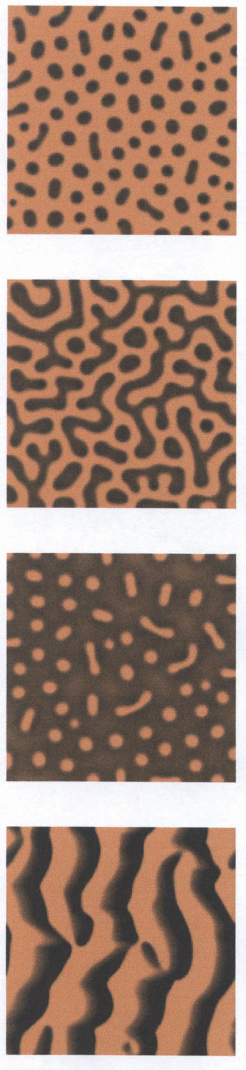
\includegraphics[height=0.7\textheight]{Figs/rietkerk2002c}\\
            \end{center}
		\end{column}				
	\end{columns} 

    \footnotesize Rietkerk et al. 2002. Am. Nat

\end{frame}

%------------------------------

\begin{frame}{Turing instabilities}

	\begin{columns}
		\begin{column}{0.5\textwidth}
            \begin{center}
                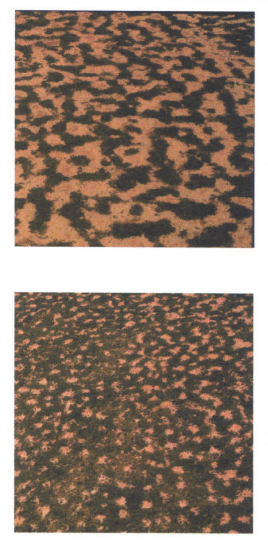
\includegraphics[height=0.6\textheight]{Figs/rietkerk2002a}\\
            \end{center}
		\end{column}
%----
		\begin{column}{0.5\textwidth}	
            \begin{center}
                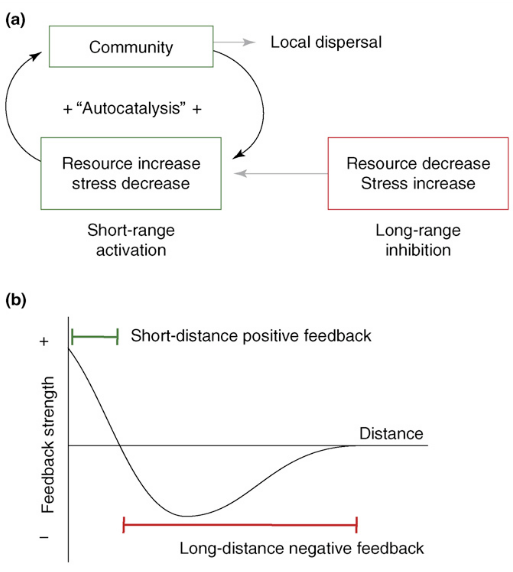
\includegraphics[height=0.6\textheight]{Figs/rietkerk2008}\\
            \end{center}
		\end{column}				
	\end{columns} 
    \footnotesize Rietkerk et al. 2002. Am. Nat

\end{frame}

%------------------------------

\begin{frame}{Patch formation in arid ecosystems }

    \begin{center}
        
\includegraphics[height=0.6\textheight]{Figs/rietkerk2004}\\
        \footnotesize Rietkerk et al. 2004. Science
    \end{center}
\end{frame}

%------------------------------
% FINAL EXERCISE
%------------------------------

{
\usebackgroundtemplate{}
\begin{frame}

	\pagecolor{BDQC1st}
	\color{white}

	\LARGE{\textit{Exercise}}

\end{frame}
}

%------------------------------

\begin{frame}{Range dynamics under global changes}

    Discuss in group how biotic interactions can affect species range shift under climate change

\end{frame}

%------------------------------
%------------------------------
\end{document}
